\documentclass{elektr}
\usepackage[all]{xy}
\usepackage{amsfonts,amssymb,amsmath,amsgen,amsopn,amsbsy,theorem,graphicx,epsfig}
\usepackage{amscd,bezier,latexsym,mathrsfs,eurosym,enumerate}
\usepackage[utf8]{inputenc}
\usepackage[english]{babel}
\usepackage{multirow}
\usepackage[dvipsnames]{xcolor}
\usepackage[pagewise]{lineno}
\usepackage{booktabs,tabularx,float,placeins}
\usepackage{algorithm}
\usepackage{algpseudocode}
\usepackage{tikz}
\usetikzlibrary{arrows.meta,positioning}
\definecolor{teal}{RGB}{0,128,128}
\definecolor{gold}{RGB}{218,165,32}
\definecolor{navy}{RGB}{0,0,128}
\newcolumntype{L}[1]{>{\raggedright\arraybackslash}p{#1}}
\newcolumntype{Y}{>{\raggedright\arraybackslash}X}
\tikzset{
box/.style={draw,rounded corners,align=center,fill=blue!5,inner sep=5pt},
arrow/.style={-{Latex[length=2mm]},thick}
}
\newcommand{\safeincludegraphics}[2][]{%
  \IfFileExists{#2}{\includegraphics[#1]{#2}}{%
    \fbox{\parbox[c][32mm][c]{0.82\linewidth}{\centering
      External figure not supplied:\\[0.4ex]\texttt{\detokenize{#2}}}}}}
\usepackage{hyperref}
\hypersetup{
colorlinks=true,
urlcolor=black,
citecolor=blue}
\usepackage{cleveref}
\makeatletter
\renewcommand{\theHALG@line}{\thealgorithm.\arabic{ALG@line}}
\makeatother
\linenumbers

\yil{}
\vol{}
\fpage{}
\lpage{}
\doi{}

\title{
An Explainable Logistic-Meta-Learner Stacking Framework with Domain-Informed Feature Engineering for Multiclass Sleep-Disorder Risk Stratification \\

}


\author[AUTHOR and AUTHOR]{
	\textbf{Md A$^{1,}$\thanks{elektrik@tubitak.gov.tr}~, Second AUTHOR$^{1,2}$}\\
 
	$^{1}$First Department, First Faculty, First University, First City, First Country\\ 	First AUTHOR: \url{https://orcid.org/0000-0001-2345-6789} \\
	$^{2}$Second Department With a Long Name, Second Faculty With a Long Name, Second University,\\ Second City, Second Country\\ Second AUTHOR: \url{https://orcid.org/0000-0001-2345-6785}\\
\\

\rec{...}
\acc{...}
\finv{...}
}

\def\E{\ifmmode{\mathbb E}\else{$\mathbb E$}\fi} %natural numbers
\def\N{\ifmmode{\mathbb N}\else{$\mathbb N$}\fi} %natural numbers
\def\R{\ifmmode{\mathbb R}\else{$\mathbb R$}\fi} %real numbers
\def\Q{\ifmmode{\mathbb Q}\else{$\mathbb Q$}\fi} %rational numbers
\def\C{\ifmmode{\mathbb C}\else{$\mathbb C$}\fi} %complex numbers
\def\H{\ifmmode{\mathbb H}\else{$\mathbb H$}\fi} %complex numbers
\def\Z{\ifmmode{\mathbb Z}\else{$\mathbb Z$}\fi} %integers
\def\P{\ifmmode{\mathbb P}\else{$\mathbb P$}\fi} %real numbers
\def\T{\ifmmode{\mathbb T}\else{$\mathbb T$}\fi} %real numbers
\def\SS{\ifmmode{\mathbb S}\else{$\mathbb S$}\fi} %real numbers
\def\DD{\ifmmode{\mathbb D}\else{$\mathbb D$}\fi} %real numbers

\renewcommand{\a}{\alpha}
\renewcommand{\b}{\beta}
\renewcommand{\d}{\delta}
\newcommand{\D}{\Delta}
\newcommand{\e}{\epsilon}
\newcommand{\var}{\varepsilon}
\newcommand{\g}{\gamma}
\newcommand{\la}{\lambda}
\newcommand{\La}{\Lambda}
\newcommand{\lan}{\langle}
\newcommand{\ran}{\rangle}
\newcommand{\n}{\nabla}
\newcommand{\va}{\varphi}
\newcommand{\s}{\sigma}
\newcommand{\Sig}{\Sigma}
\renewcommand{\t}{\tau}
\renewcommand{\th}{\theta}
\newcommand{\Om}{\Omega}
\newcommand{\om}{\omega}
\newcommand{\pa}{\partial}
\newcommand{\up}{\upsilon}
\newcommand{\vp}{\varphi}
\newcommand{\z}{\zeta}





\newcommand{\bse}{\begin{subequations}}
\newcommand{\ese}{\end{subequations}}
\newcommand{\ben}{\begin{enumerate}}
\newcommand{\een}{\end{enumerate}}
\newcommand{\bens}{\begin{enumerate*}}
\newcommand{\eens}{\end{enumerate*}}
\newcommand{\be}{\begin{equation}}
\newcommand{\ee}{\end{equation}}
\newcommand{\bea}{\begin{eqnarray}}
\newcommand{\eea}{\end{eqnarray}}
\newcommand{\baa}{\begin{eqnarray*}}
\newcommand{\eaa}{\end{eqnarray*}}
\newcommand{\bc}{\begin{center}}
\newcommand{\ec}{\end{center}}
\newcommand{\ol}{\overline}
\newcommand{\ul}{\underline}
\newcommand{\ov}{\overbrace}
\newcommand{\uv}{\underbrace}
\newcommand{\Ra}{\Rightarrow}
\newcommand{\ra}{\rightarrow}
\newcommand{\ds}{\displaystyle}
\newcommand{\vs}{\vspace}


\newcommand{\IR}{\mbox{I \hspace{-0.2cm}R}}
\newcommand{\IN}{\mbox{I \hspace{-0.2cm}N}}



%% \theoremstyle{plain} %% This is the default

\newtheorem{theorem}{Theorem}%[section]

\newtheorem{corollary}{Corollary}

\newtheorem{lemma}{Lemma}

\newtheorem{proposition}{Proposition}

\newtheorem{axiom}{Axiom}

\newtheorem{conjecture}{Conjecture}

\newtheorem{example}{Example}

\newtheorem{definition}{Definition}%[section]

\newtheorem{remark}{Remark}%[section]
\newtheorem{notation}{Notation}


\newtheorem{question}{Question}%[section]
\newtheorem{construction}{Construction}

\newtheorem{athm}{Theorem}
\renewcommand{\theathm}{\Alph{athm}}




\setcounter{page}{1}
\begin{document}
\raggedbottom

\maketitle

\begin{abstract}Accurate risk stratification may facilitate timely referral for sleep assessment, yet models developed from small tabular datasets are particularly susceptible to outcome ambiguity, preprocessing leakage, and optimistic validation. This study develops an explainable stacking framework using the publicly available Sleep Health and Lifestyle Dataset, comprising 374 participant-level observations, 11 mixed-type predictors, and three outcome categories: no recorded disorder, insomnia, and sleep apnea. Administrative identifiers were excluded, blood pressure was decomposed into systolic and diastolic components, and every data-dependent transformation was estimated exclusively from the training partition. Random Forest, XGBoost, and a radial-basis-function support vector machine were integrated as base learners through a logistic-regression meta-learner fitted to out-of-fold class probabilities and the encoded predictor pass-through. Model behaviour was examined using complementary SHAP and LIME analyses, a class-separability diagnostic based on principal component analysis, and a two-dimensional Accumulated Local Effects surface, while discrimination was assessed on a stratified 20\% hold-out set and summarised with one-vs-rest ROC--AUC. The proposed stack correctly classified 73 of 75 observations, corresponding to an accuracy of 97.33\% and a macro-F1 score of 0.96, with a macro-average ROC--AUC of 0.997. Class-specific F1 scores were 0.93 for insomnia, 1.00 for no recorded disorder, and 0.94 for sleep apnea. The RF--XGBoost soft-voting comparator achieved 93.33\% accuracy on the same partition. A repeated-split robustness check across 13 additional stratified partitions indicated a mean test accuracy of 0.924 (SD 0.027) for the proposed stack, consistent with the single-split result. These findings establish a reproducible computational benchmark rather than a clinically deployable diagnostic system. Independent outcome adjudication, repeated internal validation, calibration analysis, and prospective external evaluation remain necessary.

\keywords{sleep disorder, insomnia , sleep apnea, stacking ensemble, XGBoost, explainable machine learning ,clinical decision support}
\end{abstract}

\section{Introduction}
Sleep disorders comprise clinically heterogeneous conditions with distinct diagnostic criteria and management pathways. The 2023 text revision of the International Classification of Sleep Disorders separates insomnia disorders from sleep-related breathing disorders, whereas the benchmark used here compresses this richer taxonomy into three coarse outcome categories \cite{aasm2023}. Obstructive sleep apnea is especially relevant to screening research because conventional diagnostic pathways remain resource intensive and access to definitive testing is uneven \cite{korkalainen2024,giorgi2025,bazoukis2023}. A data-driven model may therefore assist referral prioritisation, but it cannot establish a diagnosis from lifestyle attributes alone.

Structured lifestyle and physiological data offer a pragmatic basis for methodological development, but they also create substantial analytical risk. Predictors differ in scale and representation, categorical levels require harmonisation, and the outcome classes are unequal. Performance can be materially inflated when preprocessing precedes data partitioning, model choices are adapted to evaluation results, or uncertainty from a small test sample is ignored \cite{kapoor2023,efthimiou2024,collins2024}. Reliable evaluation consequently requires strict separation of development and test data, class-sensitive metrics, paired uncertainty analysis, and explicit limits on transportability and clinical interpretation.

This study addresses these requirements through five contributions. First, it specifies an auditable preprocessing strategy for mixed numerical and categorical variables, with all learned transformations confined to the development partition. Second, it develops a heterogeneous stack in which Random Forest, XGBoost, and a radial-basis-function support vector machine contribute out-of-fold class probabilities and the encoded predictors are passed to a logistic meta-learner. Third, it evaluates the proposed model against soft voting and previously reported ANN ensembles, including a repeated-split robustness check. Fourth, it combines SHAP, LIME, a PCA-based class-separability diagnostic, and a two-dimensional Accumulated Local Effects surface to examine global importance, local attribution, and feature-interaction patterns while explicitly separating predictive association from causal or diagnostic interpretation \cite{jung2023,allen2024,pesapane2026}. Fifth, it reports one-vs-rest ROC--AUC alongside threshold-based metrics to characterise ranking quality independently of the classification threshold.

\section{Related work and study rationale}
Recent sleep-AI research has concentrated primarily on apnea detection from physiological signals and wearable devices. Contemporary reviews cover electrocardiographic, oximetric, respiratory, and multimodal signal pipelines, and consistently distinguish automated screening from clinically adjudicated diagnosis \cite{bazoukis2023,tyagi2023,abdalrazaq2024,giorgi2025}. This evidence base is informative for clinical framing but is not directly comparable with the present low-dimensional lifestyle dataset, which contains neither raw physiological waveforms nor polysomnographic severity indices.

For tabular prediction, recent evidence continues to treat tree ensembles and neural architectures as complementary rather than universally interchangeable model families \cite{borisov2024}. Alom et al. applied ANN bagging, boosting, and weighted averaging to the same sleep-health benchmark used here \cite{alom2024}; their reported accuracies provide the only literature-derived numerical comparator in this manuscript. In a different clinical setting, Alabi et al. demonstrated that heterogeneous stacking can be paired with SHAP and LIME, but their cancer-survival task, sample construction, and validation design preclude direct performance comparison \cite{alabi2023}. The unresolved methodological question is therefore whether an out-of-fold RF--XGBoost--SVM stack can improve discrimination on this specific benchmark while maintaining strict evaluation separation and transparent uncertainty.

The explanation layer is deliberately bounded. Recent reviews emphasise that post-hoc explanations require explicit definitions of audience, fidelity, stability, and intended use; an attribution is evidence about a fitted prediction function, not a causal mechanism or clinical rationale \cite{jung2023,allen2024}. Likewise, current reporting and deployment guidance requires transparent data provenance, evaluation design, uncertainty, and validation before clinical use \cite{tripodai2024,futureai2025}. Accordingly, all ANN percentages in the comparative table are transcribed from Alom et al. \cite{alom2024}, whereas every RF--XGBoost--SVM value is generated by the present analysis. The comparison is descriptive because the studies do not share an identical evaluation protocol.
\begin{table}[H]
\centering
\caption{Summary of related studies and their relevance to this work.}
\label{tab:related_work}
\small
\setlength{\tabcolsep}{4pt}
\renewcommand{\arraystretch}{1.05}
\begin{tabularx}{\textwidth}{@{}L{0.18\textwidth}L{0.22\textwidth}L{0.23\textwidth}Y@{}}
\toprule
Study & Data/task & Methods & Relevance \\
\midrule

Alom et al. \cite{alom2024} &
Sleep-health tabular data &
ANN Ensembles &
Main Numerical Comparator \\

Alabi et al. \cite{alabi2023} &
Cancer survival &
Stacking, SHAP, LIME &
Supports explainable stacking \\

Bazoukis et al. \cite{bazoukis2023} &
Physiological sleep data &
ML/DL methods &
Clinical screening context \\

Tyagi et al. \cite{tyagi2023} &
Sleep signals &
ML/DL pipelines &
Signal-based comparison \\

Borisov et al. \cite{borisov2024} &
Tabular datasets &
Tree and neural models &
Supports heterogeneous models \\

\textbf{This study} &
\textbf{Sleep-Health Tabular Data} &
\textbf{RF--XGBoost--SVM stack} &
\textbf{TVLE + XAI + Uncertainty} \\

\bottomrule
\end{tabularx}
\end{table}

\section{Materials and methods}
\subsection{Methodological overview}
The investigation followed a leakage-controlled analytical pathway (Fig.~\ref{fig:workflow}). Data integrity and outcome coding were examined before modelling, after which the administrative identifier was removed and clinically interpretable features were derived. A stratified test partition was then isolated prior to fitting any transformation. Within the development partition, numerical variables were standardised, categorical variables were one-hot encoded, and out-of-fold probability estimates were generated for all three base learners. These estimates and the encoded predictors formed the input to a logistic-regression meta-learner through the implemented pass-through connection. Final discrimination, paired model comparisons, and explanation analyses were conducted only after the complete pipeline had been fixed. This design preserves the independence of the test set and prevents information from the evaluation sample from influencing representation learning or model construction.

\begin{figure}[H]
\centering
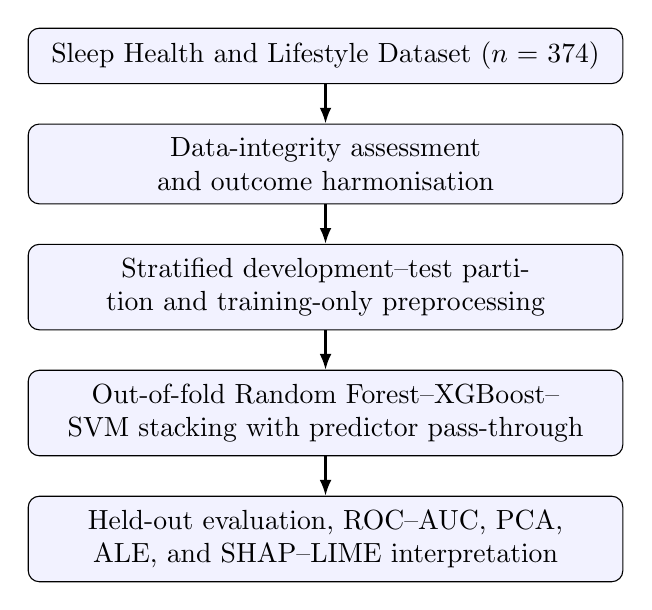
\begin{tikzpicture}[node distance=5mm]
\node[box,text width=72mm] (d) {Sleep Health and Lifestyle Dataset ($n=374$)};
\node[box,text width=72mm,below=of d] (a) {Data-integrity assessment and outcome harmonisation};
\node[box,text width=72mm,below=of a] (p) {Stratified development--test partition and training-only preprocessing};
\node[box,text width=72mm,below=of p] (m) {Out-of-fold Random Forest--XGBoost--SVM stacking with predictor pass-through};
\node[box,text width=72mm,below=of m] (e) {Held-out evaluation, ROC--AUC, PCA, ALE, and SHAP--LIME interpretation};
\draw[arrow] (d)--(a);
\draw[arrow] (a)--(p);
\draw[arrow] (p)--(m);
\draw[arrow] (m)--(e);
\end{tikzpicture}
\caption{Study design and analytical workflow. The held-out test partition remains isolated from feature transformation, base-learner estimation, and meta-learner construction until final evaluation.}
\label{fig:workflow}
\end{figure}

\subsection{Problem formulation and notation}
Let the benchmark sample be $\mathcal{D}=\{(\mathbf{x}_i,y_i)\}_{i=1}^{N}$, where $N=374$, $\mathbf{x}_i\in\mathbb{R}^{d_n}\times\mathcal{A}^{d_c}$ contains numerical and categorical predictors, and $y_i\in\mathcal{C}=\{0,1,2\}$ denotes insomnia, no recorded disorder, or sleep apnea. The analytical objective is to estimate a probabilistic mapping
\begin{equation}
F:\mathcal{X}\rightarrow\Delta^{C-1},\qquad
\hat y_i=\arg\max_{c\in\mathcal{C}}F_c(\mathbf{x}_i),
\label{eq:problem}
\end{equation}
where $C=3$ and $\Delta^{C-1}$ is the probability simplex. The stratified partition satisfies
\begin{equation}
\mathcal{D}_{tr}\cap\mathcal{D}_{te}=\varnothing,
\qquad |\mathcal{D}_{tr}|=299,
\qquad |\mathcal{D}_{te}|=75,
\label{eq:partition}
\end{equation}
and every estimated parameter is a function of $\mathcal{D}_{tr}$ only. For numerical predictor $j$, development-set standardisation is
\begin{equation}
\widetilde{x}_{ij}=\frac{x_{ij}-\mu^{(tr)}_j}{\sigma^{(tr)}_j},
\quad
\mu^{(tr)}_j=\frac{1}{n_{tr}}\sum_{i\in\mathcal{D}_{tr}}x_{ij},
\label{eq:standardise}
\end{equation}
where $\sigma^{(tr)}_j$ is the sample standard deviation estimated from $\mathcal{D}_{tr}$. A categorical level $a_q$ is represented by $o_{iq}=\mathbb{I}(x_{ij}=a_q)$. Consequently, the fitted transformer $T_{\widehat{\theta}_{tr}}$ maps each observation to the fixed-schema vector $\mathbf{x}'_i=T_{\widehat{\theta}_{tr}}(\mathbf{x}_i)$, with neither the scale parameters nor the categorical vocabulary re-estimated on the test partition.

\subsection{Data source and outcome definition}
The analysis used the publicly available Sleep Health and Lifestyle Dataset hosted on Kaggle \cite{kaggle2023}. The dataset comprises 374 participant-level observations and 13 variables: one administrative identifier, 11 candidate predictors, and the Sleep Disorder outcome. The predictors represent demographic characteristics, sleep behaviour, physical activity, perceived stress, body-mass category, heart rate, and blood pressure. Because the data were not collected as a prospectively recruited clinical cohort and the outcome was not independently adjudicated, the dataset is treated as a methodological benchmark for risk stratification rather than as a source of prevalence estimates or diagnostic ground truth.

All 11 predictors were complete, whereas 219 outcome entries were blank. Consistent with the coding used in the analytical dataset, blank outcomes were assigned to the no-recorded-disorder category, producing 219 observations with no recorded disorder, 77 with insomnia, and 78 with sleep apnea. This operational definition is consequential because absence of a recorded label is not equivalent to clinician-confirmed absence of disease. The assignment was therefore retained for reproducibility but treated as a primary source of outcome uncertainty throughout interpretation.

\begin{table}[ht]
\centering
\caption{Descriptive characteristics of the 374 observations used for model development and evaluation.}
\label{tab:datasetprofile}
\small
\setlength{\tabcolsep}{5pt}
\renewcommand{\arraystretch}{1.05}
\begin{tabularx}{\textwidth}{@{}L{0.25\textwidth}L{0.27\textwidth}Y@{}}
\toprule
Profile item & Observed value & Interpretation \\
\midrule
Records and variables & 374 records; 13 variables & Person-level tabular benchmark \\
Candidate predictors & 11 & Mixed numerical and categorical fields \\
Outcome completeness & 155 labelled; 219 blank & Blank entries mapped to no recorded disorder \\
Class distribution & No recorded disorder, 219; insomnia, 77; sleep apnea, 78 & Unequal class frequencies \\
Age & 27--59 years; mean, 42.18 & Demographic predictor \\
Sleep duration & 5.8--8.5 h; mean, 7.13 h & Self-reported sleep behaviour \\
Heart rate & 65--86 bpm; mean, 70.17 bpm & Physiological indicator \\
Daily steps & 3,000--10,000; mean, 6,816.84 & Activity indicator \\
Categorical levels & Gender, 2; occupation, 11; BMI, 4 & Harmonised before one-hot encoding \\
\bottomrule
\end{tabularx}
\end{table}

Age ranged from 27 to 59 years (mean 42.18, standard deviation 8.67), and reported sleep duration ranged from 5.8 to 8.5 h (mean 7.13, standard deviation 0.80). Quality-of-sleep scores ranged from 4 to 9, physical-activity levels from 30 to 90, stress scores from 3 to 8, heart rate from 65 to 86 beats/min, and daily step counts from 3,000 to 10,000. The categorical variables comprised two gender categories, 11 occupational groups, and four body-mass-index labels. Blood pressure, originally represented as a systolic/diastolic string, was separated into two numerical variables. The synonymous labels ``Normal Weight'' and ``Normal'' were consolidated before one-hot encoding.

\begin{table}[ht]
\centering
\caption{Predictor groups, representative variables, and their computational treatment within the modelling pipeline.}
\label{tab:variables}
\small
\begin{tabular}{L{0.24\linewidth}L{0.25\linewidth}L{0.42\linewidth}}
\toprule
Variable group & Examples & Treatment \\
\midrule
Administrative & Person ID & Removed before modelling \\
Demographic & Age, Gender, Occupation & Categorical encoding; age standardisation \\
Sleep behaviour & Sleep Duration, Quality of Sleep & Numerical standardisation \\
Lifestyle & Physical Activity Level, Daily Steps & Numerical standardisation \\
Psychophysiological & Stress Level, Heart Rate & Numerical standardisation \\
Anthropometric & BMI Category & Category harmonisation and one-hot encoding \\
Cardiovascular & Blood Pressure & Split into systolic and diastolic values \\
Target & Sleep Disorder & Label encoding into three classes \\
\bottomrule
\end{tabular}
\end{table}

Person ID was excluded because it contains ordering information without a plausible physiological interpretation. Occupation was retained as a contextual predictor, although its contribution requires careful scrutiny because it may encode socioeconomic structure and introduce transportability concerns. The public-source provenance, modest sample size, outcome-assignment rule, and absence of clinical adjudication therefore define the inferential boundaries of this study.

\begin{figure}[ht]
\centering
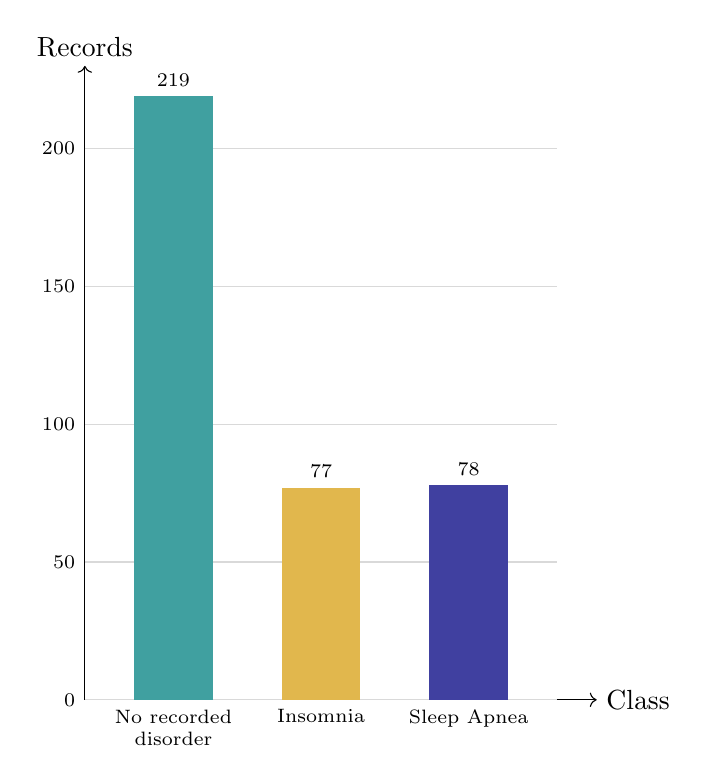
\begin{tikzpicture}[x=1.25cm,y=0.035cm]
\draw[->] (0,0)--(5.2,0) node[right]{Class};
\draw[->] (0,0)--(0,230) node[above]{Records};
\foreach \y in {0,50,100,150,200}{\draw[gray!30] (0,\y)--(4.8,\y);\node[left,font=\scriptsize] at (0,\y){\y};}
\fill[teal!75] (0.5,0) rectangle (1.3,219);\fill[gold!80] (2.0,0) rectangle (2.8,77);\fill[navy!75] (3.5,0) rectangle (4.3,78);
\node[above,font=\scriptsize] at (0.9,219){219};\node[above,font=\scriptsize] at (2.4,77){77};\node[above,font=\scriptsize] at (3.9,78){78};
\node[below,align=center,font=\scriptsize] at (0.9,0){No recorded\\disorder};\node[below,font=\scriptsize] at (2.4,0){Insomnia};\node[below,font=\scriptsize] at (3.9,0){Sleep Apnea};
\end{tikzpicture}
\caption{Outcome distribution after harmonisation. Blank outcome entries were assigned to no recorded disorder, yielding 219 observations with no recorded disorder, 77 with insomnia, and 78 with sleep apnea.}
\label{fig:distribution}
\end{figure}


\subsection{Class separability diagnostic (PCA)}
\label{sec:pca}
To characterise the intrinsic separability of the three outcome classes independent of any specific classifier, a two-component principal component analysis was fitted to the fully preprocessed (scaled and one-hot encoded) feature matrix using all 374 observations. This projection is diagnostic only: it is fitted separately from, and never substituted into, the classification pipeline described in Sections~3.5--3.6, so it does not affect any reported classification metric.

The first two components explained 33.68\% and 29.47\% of total variance respectively (63.14\% combined), indicating that a large share of the feature-space structure is not captured in two dimensions and that any apparent overlap in the projection understates the information available to the full-dimensional classifiers. Fig.~\ref{fig:pca}a shows the raw two-dimensional scatter, and Fig.~\ref{fig:pca}b overlays 1-sigma covariance ellipses per class. The no-recorded-disorder class occupies a visually distinct region, consistent with its perfect recall in Table~\ref{tab:metrics}, whereas the insomnia and sleep-apnea ellipses show partial overlap. This is consistent with, though not a direct explanation for, the two insomnia-to-apnea misclassifications reported in Section~5 and discussed in Section~7.

\begin{figure}[H]
\centering
\safeincludegraphics[width=\linewidth]{pca_class_separability.png}
\caption{PCA projection of the preprocessed feature space (diagnostic only, not part of the modelling pipeline): (a) raw scatter by outcome class; (b) the same projection with 1-sigma class ellipses. PC1 and PC2 explain 33.68\% and 29.47\% of variance, respectively.}
\label{fig:pca}
\end{figure}

\FloatBarrier

\subsection{Data splitting and leakage control}
An 80:20 stratified partition with random seed 42 produced a development set of 299 observations and an independent test set of 75 observations. The split was performed before numerical scaling, categorical encoding, or model fitting. All preprocessing parameters---including numerical means and variances, categorical vocabularies, and label mappings---were estimated from the development data and subsequently applied without modification to the test set. The same principle was maintained within cross-validation folds used to construct the stack. This ordering prevents evaluation-set information from influencing either the feature representation or the fitted decision function \cite{kapoor2023,efthimiou2024}.

\begin{algorithm}[H]
\caption{Leakage-controlled preparation of development and test partitions}
\label{alg:prep}
\begin{algorithmic}[1]
\Require Dataset $D$, target $y$, seed $s=42$
\Ensure Transformed partitions $(X'_{tr},y_{tr})$ and $(X'_{te},y_{te})$
\State Remove identifier fields and assign blank outcomes to no recorded disorder
\State Harmonise BMI labels and split Blood Pressure into two integers
\State Perform an 80:20 stratified split using seed $s$
\State Fit the scaler and one-hot encoder on $X_{tr}$ only
\State Transform $X_{tr}$ and $X_{te}$ using the fitted objects
\State Fit the label map on $y_{tr}$ and apply it to $y_{te}$
\State \Return $(X'_{tr},y_{tr})$, $(X'_{te},y_{te})$
\end{algorithmic}
\end{algorithm}

\begin{figure}[H]
\centering
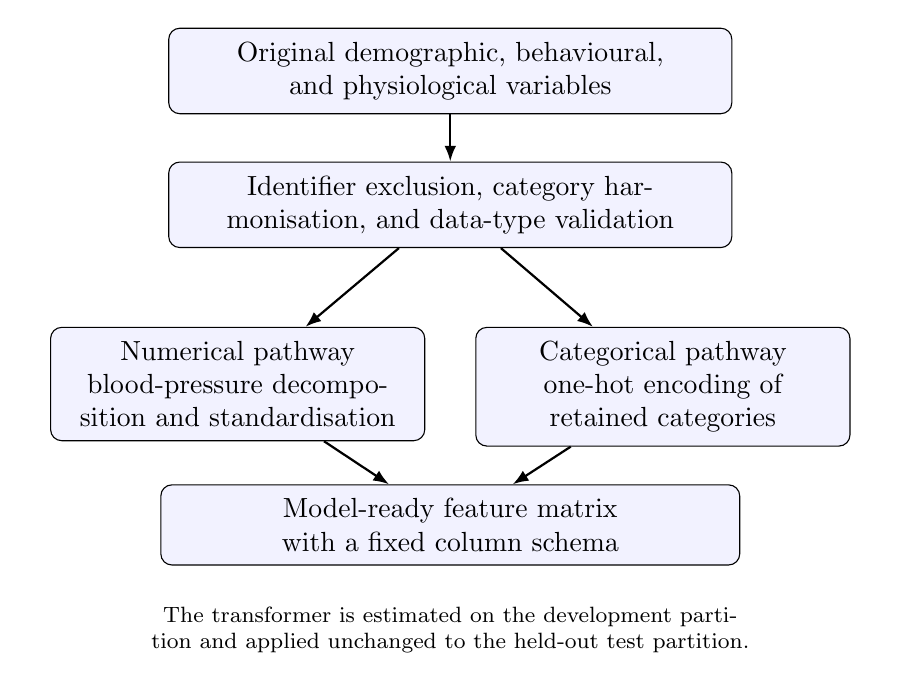
\begin{tikzpicture}[node distance=6mm and 8mm]
\node[box,text width=68mm] (raw) {Original demographic, behavioural, and physiological variables};
\node[box,text width=68mm,below=of raw] (audit) {Identifier exclusion, category harmonisation, and data-type validation};
\node[box,text width=44mm,below=10mm of audit,xshift=-27mm] (num) {Numerical pathway\\blood-pressure decomposition and standardisation};
\node[box,text width=44mm,below=10mm of audit,xshift=27mm] (cat) {Categorical pathway\\one-hot encoding of retained categories};
\node[box,text width=70mm,below=30mm of audit] (out) {Model-ready feature matrix with a fixed column schema};
\draw[arrow] (raw)--(audit);
\draw[arrow] (audit)--(num);
\draw[arrow] (audit)--(cat);
\draw[arrow] (num)--(out);
\draw[arrow] (cat)--(out);
\node[below=4mm of out,align=center,text width=105mm,font=\footnotesize] {The transformer is estimated on the development partition and applied unchanged to the held-out test partition.};
\end{tikzpicture}
\caption{Leakage-controlled feature-engineering pipeline. Numerical and categorical transformations are estimated exclusively from the development partition and applied unchanged to the held-out test partition.}
\label{fig:preprocess}
\end{figure}

\FloatBarrier

\subsection{Base learners and stacking design}
The proposed architecture combines three base learners with complementary bias--variance and margin-based characteristics. The Random Forest comprised 200 trees with random seed 42 (scikit-learn default depth and split settings). For $B$ fitted trees, its class probability is the average tree vote
\begin{equation}
p_{RF}(c\mid\mathbf{x}')=\frac{1}{B}\sum_{b=1}^{B}
\mathbb{I}\!\left(h_b(\mathbf{x}')=c\right).
\label{eq:rf}
\end{equation}
XGBoost used 200 boosting iterations, a learning rate of 0.05, and maximum depth 5. Its class-specific additive score and corresponding probability can be written as
\begin{equation}
s_c^{(M)}(\mathbf{x}')=\sum_{m=1}^{M}\eta f_{mc}(\mathbf{x}'),
\qquad
p_{XGB}(c\mid\mathbf{x}')=
\frac{\exp(s_c^{(M)})}{\sum_{r=1}^{C}\exp(s_r^{(M)})}.
\label{eq:xgb}
\end{equation}
A radial-basis-function support vector machine with probability calibration (Platt scaling) was included as a third, margin-based base learner, contributing class-probability estimates $p_{SVM}(c\mid\mathbf{x}')$ in the same format as the two tree-based learners. Its inclusion is intended to capture decision-boundary geometry that neither bagged nor boosted trees represent directly.

For each observation in the development set, five-fold cross-validation generated probabilities from models that excluded that observation during fitting. If $\kappa(i)$ denotes the fold containing observation $i$, the meta-level vector is
\begin{equation}
\mathbf{z}^{OOF}_i=\left[\,{\mathbf{x}'_i}^{\!\top},\
{\mathbf{p}_{RF}^{(-\kappa(i))}(\mathbf{x}'_i)}^{\!\top},\
{\mathbf{p}_{XGB}^{(-\kappa(i))}(\mathbf{x}'_i)}^{\!\top},\
{\mathbf{p}_{SVM}^{(-\kappa(i))}(\mathbf{x}'_i)}^{\!\top}\right]^{\!\top}
\in\mathbb{R}^{d+3C}.
\label{eq:oofvector}
\end{equation}
The inclusion of $\mathbf{x}'_i$ represents the implemented pass-through connection. A multinomial logistic meta-learner then estimates
\begin{equation}
p_{S}(c\mid\mathbf{z})=
\frac{\exp(\beta_{c0}+\boldsymbol{\beta}_c^{\top}\mathbf{z})}
{\sum_{r=1}^{C}\exp(\beta_{r0}+\boldsymbol{\beta}_r^{\top}\mathbf{z})},
\label{eq:meta}
\end{equation}
by minimising regularised multiclass log loss
\begin{equation}
\widehat{\boldsymbol{\beta}}=
\arg\min_{\boldsymbol{\beta}}
\left[-\frac{1}{n_{tr}}\sum_{i=1}^{n_{tr}}\sum_{c=1}^{C}
\mathbb{I}(y_i=c)\log p_S(c\mid\mathbf{z}^{OOF}_i)
+\lambda_{\beta}\sum_{c=1}^{C}\lVert\boldsymbol{\beta}_c\rVert_2^2\right].
\label{eq:metaloss}
\end{equation}
Here, $\lambda_{\beta}$ denotes the L2 penalty governed by the implementation's inverse-regularisation setting $C_{\mathrm{LR}}=0.3$. The base models were subsequently refitted on the full development set for inference on unseen observations. Restricting meta-learner training to out-of-fold predictions is essential; using in-sample probabilities would expose the second level to optimistically biased representations \cite{kapoor2023,alabi2023}.

\begin{table}[H]
\centering
\caption{Hyperparameter configuration of the Random Forest, XGBoost, and SVM base learners, the logistic-regression meta-learner, and the validation split.}
\label{tab:hyper}
\small
\begin{tabular}{lll}
\toprule
Component & Parameter & Value \\
\midrule
Random Forest & number of trees & 200 \\
 & random seed & 42 \\
XGBoost & estimators / learning rate & 200 / 0.05 \\
 & maximum depth & 5 \\
SVM & kernel & RBF \\
 & probability calibration & enabled (Platt scaling) \\
Meta-learner & model & logistic regression \\
 & inverse regularisation / solver & $C_{\mathrm{LR}}=0.3$ / L-BFGS \\
 & encoded-feature pass-through & enabled \\
Validation & split / seed & 80:20 stratified / 42 \\
 & stacking folds & 5 \\
\bottomrule
\end{tabular}
\end{table}

\begin{figure}[H]
\centering
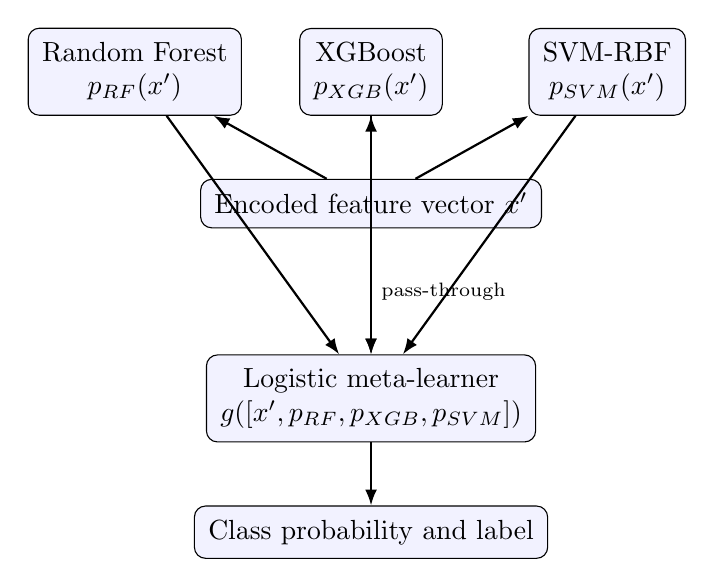
\begin{tikzpicture}[node distance=8mm and 12mm]
\node[box] (x) {Encoded feature vector $x'$};
\node[box,above=8mm of x,xshift=-30mm] (rf) {Random Forest\\$p_{RF}(x')$};
\node[box,above=8mm of x] (xgb) {XGBoost\\$p_{XGB}(x')$};
\node[box,above=8mm of x,xshift=30mm] (svm) {SVM-RBF\\$p_{SVM}(x')$};
\node[box,below=16mm of x] (meta) {Logistic meta-learner\\$g([x',p_{RF},p_{XGB},p_{SVM}])$};
\node[box,below=of meta] (y) {Class probability and label};
\draw[arrow] (x)--(rf);\draw[arrow] (x)--(xgb);\draw[arrow] (x)--(svm);
\draw[arrow] (rf)--(meta);\draw[arrow] (xgb)--(meta);\draw[arrow] (svm)--(meta);
\draw[arrow,dashed] (x)--node[right,font=\scriptsize]{pass-through} (meta);\draw[arrow] (meta)--(y);
\end{tikzpicture}
\caption{Architecture of the proposed heterogeneous stack. Out-of-fold Random Forest, XGBoost, and SVM-RBF class-probability vectors are concatenated with the encoded predictors through the pass-through connection; the logistic meta-learner then estimates the final multiclass probabilities.}
\label{fig:stack}
\end{figure}

\begin{algorithm}[H]
\caption{Leakage-controlled out-of-fold stacking and held-out inference}
\label{alg:stack}
\small
\begin{algorithmic}[1]
\Require $(X'_{tr},y_{tr})$, transformed test vector $x'$, $K=5$ folds
\Ensure Predicted class $\hat y$
\For{$k=1$ to $K$}
\State Fit $f_{RF}^{(-k)}$, $f_{XGB}^{(-k)}$, and $f_{SVM}^{(-k)}$ outside fold $k$
\State Store probabilities on fold $k$ as $P_{RF}^{(k)}$, $P_{XGB}^{(k)}$, $P_{SVM}^{(k)}$
\EndFor
\State Form $Z=[X'_{tr},P_{RF},P_{XGB},P_{SVM}]$ using the pass-through predictors
\State Fit logistic meta-learner $g$ on $(Z,y_{tr})$ with $C_{\mathrm{LR}}=0.3$
\State Fit all three base learners on all $X'_{tr}$
\State $\hat y\gets\arg\max_c g([x',f_{RF}(x'),f_{XGB}(x'),f_{SVM}(x')])_c$
\State \Return $\hat y$
\end{algorithmic}
\end{algorithm}

\begin{figure}[H]
\centering
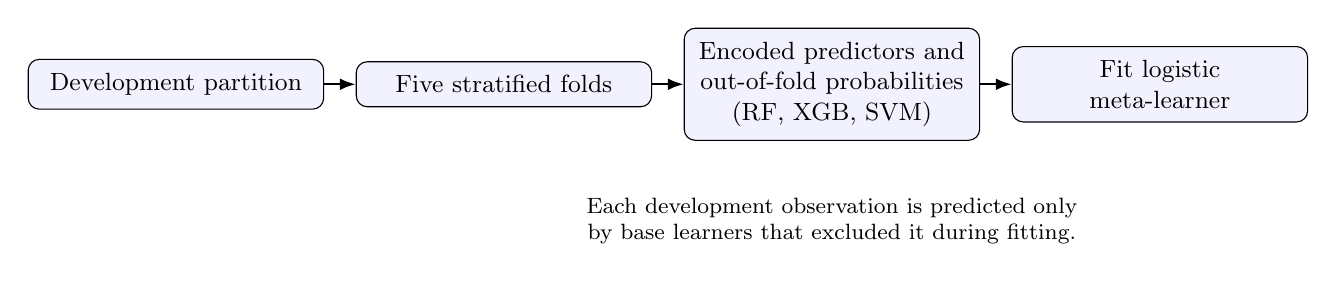
\begin{tikzpicture}[node distance=4mm,every node/.append style={font=\small,text width=34mm}]
\node[box] (d) {Development partition};
\node[box,right=of d] (f) {Five stratified folds};
\node[box,right=of f] (o) {Encoded predictors and out-of-fold probabilities (RF, XGB, SVM)};
\node[box,right=of o] (l) {Fit logistic meta-learner};
\draw[arrow] (d)--(f);\draw[arrow] (f)--(o);\draw[arrow] (o)--(l);
\node[below=6mm of o,align=center,text width=95mm,font=\footnotesize] {Each development observation is predicted only by base learners that excluded it during fitting.};
\end{tikzpicture}
\caption{Construction of the meta-learner training matrix. Encoded predictors are passed through, while the probability components from all three base learners are generated out of fold to prevent second-level fitting on in-sample base-learner predictions.}
\label{fig:oof}
\end{figure}

\FloatBarrier

\subsection{Baseline soft-voting comparator}
To contextualise the proposed stack, a soft-voting ensemble combining a Random Forest (200 trees) and an XGBoost classifier (200 estimators, learning rate 0.05, maximum depth 5) was fitted as a baseline comparator, using the same fitted preprocessing pipeline described in Section~3.5. Rather than routing base-learner probabilities through a trained meta-learner, soft voting averages the predicted class probabilities of the two base learners directly, providing a simpler, non-learned alternative against which the benefit of the logistic meta-learner and the third (SVM) base learner can be assessed.

\begin{algorithm}[H]
\caption{Soft-voting ensemble using Random Forest and XGBoost}
\label{alg:voting}
\begin{algorithmic}[1]
\Require Preprocessed training data $(X_{train}, y_{train})$, test data $X_{test}$
\Ensure Predicted sleep-disorder labels $\hat{y}$
\State Initialize Random Forest classifier $RF$ with 200 trees and random seed 42
\State Initialize XGBoost classifier $XGB$ with 200 estimators, learning rate $0.05$, maximum depth $5$, and \texttt{mlogloss} objective
\State Create soft-voting ensemble:
\[
V = \operatorname{SoftVote}(RF, XGB)
\]
\State Construct pipeline $\mathcal{M} = \operatorname{Pipeline}(\mathcal{P}, V)$
\State Train $\mathcal{M}$ using $(X_{train}, y_{train})$
\For{each test instance $x \in X_{test}$}
    \State Obtain class probabilities $p_{RF}(x)$ and $p_{XGB}(x)$
    \State Compute ensemble probability:
    \[
    p_V(x) = \frac{p_{RF}(x) + p_{XGB}(x)}{2}
    \]
    \State $\hat{y}(x) \gets \arg\max_c p_V(x)_c$
\EndFor
\State Evaluate $\hat{y}$ using accuracy, precision, recall, F1-score, and confusion matrix
\State \Return $\hat{y}$
\end{algorithmic}
\end{algorithm}

This comparator is reported throughout Section~5 (Tables~\ref{tab:basecomparison} and~\ref{tab:stats}, Fig.~\ref{fig:confusions}) alongside the proposed stack.

\FloatBarrier

\subsection{Explainability and auditability}
SHAP explanations were obtained through a permutation-based, model-agnostic interface. A fixed background sample $B$ was drawn exclusively from the development partition, and each perturbed observation was passed through the complete preprocessing and prediction pipeline. For class $c$, local additive consistency satisfies
\begin{equation}
F_c(\mathbf{x}_i)-\mathbb{E}_{\mathbf{X}\sim B}[F_c(\mathbf{X})]
=\sum_{j=1}^{d}\phi_{ij}^{(c)},
\label{eq:shaplocal}
\end{equation}
and global importance for feature $j$ was defined as
\begin{equation}
I_j=\frac{1}{nC}\sum_{i=1}^{n}\sum_{c=1}^{C}|\phi_{ij}^{(c)}|.
\label{eq:shapglobal}
\end{equation}
Here, $\phi_{ij}^{(c)}$ denotes the attribution assigned to feature $j$ for observation $i$ and class $c$. LIME was used as a complementary local analysis. Given perturbed neighbourhood $\mathcal{Z}_i$, proximity kernel $\pi_i$, and interpretable surrogate family $\mathcal{G}$, the local explanation is
\begin{equation}
g_i^{*}=\arg\min_{g\in\mathcal{G}}
\left\{\sum_{\mathbf{z}\in\mathcal{Z}_i}\pi_i(\mathbf{z})
[F_c(\mathbf{z})-g(\mathbf{z})]^2+\Omega(g)\right\},
\label{eq:lime}
\end{equation}
where $\Omega(g)$ penalises surrogate complexity. Absolute LIME coefficients were aggregated only to assess broad agreement with SHAP rankings; they were not treated as a second estimate of causal importance. Both methods characterise the fitted prediction function, and their outputs depend on the chosen background distribution, perturbation mechanism, and representation of predictor dependence \cite{instanceshap2023,jung2023}.

\begin{algorithm}[H]
\caption{Permutation-SHAP procedure for global model auditing}
\label{alg:shap}
\begin{algorithmic}[1]
\Require Fitted model $F$, training matrix $X_{tr}$, explanation sample $X_e$
\Ensure Ranked importance vector $I$
\State Sample a fixed background $B\subset X_{tr}$
\State Define $h(z)=F(\operatorname{decode}(z))$
\State Initialise a permutation explainer with $h$ and $B$
\State Compute $\Phi$ for $X_e$
\State $I_j\gets\operatorname{mean}_{i,c}(|\Phi_{ij}^{(c)}|)$ for each feature $j$
\State Rank features by decreasing $I_j$
\State \Return $I$
\end{algorithmic}
\end{algorithm}

\begin{figure}[t]
\centering
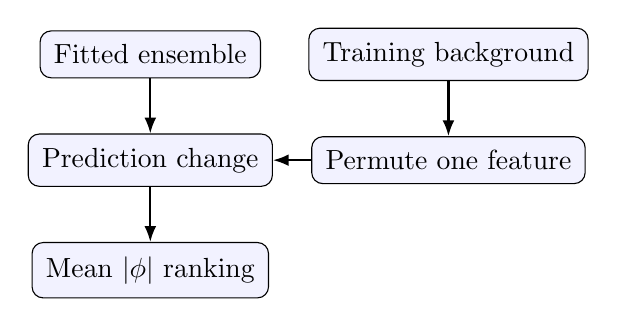
\begin{tikzpicture}[node distance=7mm and 6mm]
\node[box] (f) {Fitted ensemble};
\node[box,right=of f] (b) {Training background};
\node[box,below=of b] (p) {Permute one feature};
\node[box,below=of f] (q) {Prediction change};
\node[box,below=of q] (r) {Mean $|\phi|$ ranking};
\draw[arrow] (f)--(q);\draw[arrow] (b)--(p);\draw[arrow] (p)--(q);\draw[arrow] (q)--(r);
\end{tikzpicture}
\caption{Model-agnostic explanation workflow. Perturbations are evaluated through the complete fitted pipeline and aggregated as mean absolute feature attributions.}
\label{fig:shap}
\end{figure}

\FloatBarrier

\subsection{Feature relationships and stacking-model local effects}
\label{sec:ale}
Two additional diagnostics were used to examine dependence structure among predictors and the fitted stack's local behaviour. First, Spearman rank correlation was computed across the nine numerical predictors on the development partition, to characterise monotonic association independent of the standardisation applied in Eq.~\eqref{eq:standardise}. Second, a two-dimensional Accumulated Local Effects (ALE) surface was computed directly from the fitted stacking pipeline for the joint effect of Sleep Duration and Quality of Sleep on the predicted probability of insomnia, using a $6\times6$ quantile grid. Unlike SHAP, ALE conditions on the local data density and is therefore less sensitive to feature correlation when estimating joint effects; it was accumulated by summing corner-difference finite effects across grid cells and centring the resulting surface to zero mean.

Fig.~\ref{fig:relationships}a shows that Sleep Duration and Quality of Sleep are strongly positively correlated, while Stress Level is negatively correlated with both, consistent with their combined appearance among the higher-ranked SHAP features in Section~3.7 and Section~5.3. Fig.~\ref{fig:relationships}b shows the corresponding ALE surface: the predicted insomnia probability rises most sharply in the region of short sleep duration combined with low sleep quality, and flattens once both variables exceed their sample medians, indicating a joint rather than additive relationship between these two predictors and the insomnia class score. As with SHAP and LIME, the ALE surface characterises the fitted function's local behaviour and should not be read as a causal dose-response relationship.

\begin{figure}[H]
\centering
\safeincludegraphics[width=0.98\linewidth]{feature_relationships_ale.png}
\caption{(a) Spearman rank correlation among numerical predictors on the development partition. (b) Two-dimensional Accumulated Local Effects surface for Sleep Duration and Quality of Sleep on the stacking classifier's predicted probability of insomnia.}
\label{fig:relationships}
\end{figure}

\FloatBarrier
\section{Experimental protocol}
The evaluation used the isolated 75-observation test partition. Accuracy was reported alongside class-specific precision, recall, and F1 score, as well as macro- and support-weighted summaries. For class $c$, the principal relationships were
\begin{equation}
\begin{aligned}
P_c&=\frac{TP_c}{TP_c+FP_c}, &
R_c&=\frac{TP_c}{TP_c+FN_c},\\
F1_c&=\frac{2P_cR_c}{P_c+R_c},
\end{aligned}
\label{eq:classmetrics}
\end{equation}
with
\begin{equation}
\operatorname{Accuracy}=\frac{1}{n_{te}}\sum_{i=1}^{n_{te}}\mathbb{I}(\hat y_i=y_i),
\qquad
F1_{macro}=\frac{1}{C}\sum_{c=1}^{C}F1_c.
\label{eq:aggregatemetrics}
\end{equation}
Macro-F1 was emphasised because it assigns equal weight to each outcome category despite unequal class frequencies. One-vs-rest ROC--AUC was additionally computed from the predicted class probabilities to summarise ranking quality independently of the classification threshold, using
\begin{equation}
\operatorname{AUC}_c=\int_0^1 \mathrm{TPR}_c(\mathrm{FPR}_c^{-1}(t))\,dt,
\qquad
\operatorname{AUC}_{macro}=\frac{1}{C}\sum_{c=1}^{C}\operatorname{AUC}_c.
\label{eq:auc}
\end{equation}
The proposed stack and soft-voting comparator were additionally evaluated through paired bootstrap resampling of test observations. For bootstrap sample $b$, the paired effect was
\begin{equation}
\Delta^{(b)}=\operatorname{Accuracy}^{(b)}_{stack}
-\operatorname{Accuracy}^{(b)}_{vote},
\label{eq:bootstrap}
\end{equation}
and the 2.5th and 97.5th percentiles of $\{\Delta^{(b)}\}$ formed the 95\% interval. An exact McNemar test used only the discordant prediction counts between the two models on the identical test partition. As a further robustness check, the complete stacking pipeline was refitted across 13 additional stratified 80:20 splits (Section~6.1) to assess sensitivity to the specific partition used for the primary evaluation. The analysis assesses discrimination within the available benchmark; it does not substitute for repeated internal validation, probability calibration, subgroup analysis, or evaluation in an untouched external cohort \cite{collins2024,riley2024,rileysample2024}.

\section{Results}
The proposed stacking model correctly classified 73 of 75 test observations, yielding an accuracy of 97.33\% and a macro-F1 score of 0.96. It identified 13 of 15 insomnia observations, all 44 observations with no recorded disorder, and all 16 sleep-apnea observations. Both errors involved insomnia being classified as sleep apnea; no observation was incorrectly assigned to the no-recorded-disorder category. The RF--XGBoost soft-voting comparator achieved 93.33\% accuracy and a macro-F1 score of 0.90 on the same test set.

\begin{table}[t]
\centering
\caption{Class-specific and aggregate predictive performance of the proposed stack on the 75-observation hold-out set.}
\label{tab:metrics}
\small
\begin{tabular}{lrrrr}
\toprule
Class/model & Precision & Recall & F1 & Support \\
\midrule
Insomnia & 1.00 & 0.87 & 0.93 & 15 \\
No recorded disorder & 1.00 & 1.00 & 1.00 & 44 \\
Sleep Apnea & 0.89 & 1.00 & 0.94 & 16 \\
Macro average & 0.96 & 0.96 & 0.96 & 75 \\
Weighted average & 0.98 & 0.97 & 0.97 & 75 \\
\midrule
Soft voting macro average & 0.90 & 0.91 & 0.90 & 75 \\
\bottomrule
\end{tabular}
\end{table}

\subsection{Discrimination via ROC--AUC}
\label{sec:rocauc}
One-vs-rest ROC--AUC was computed on the same 75-observation test partition to assess ranking quality independent of the classification threshold implicit in Table~\ref{tab:metrics}. Per-class AUC was 0.994 for insomnia, 1.000 for no recorded disorder, and 0.997 for sleep apnea, giving a macro-average ROC--AUC of 0.997 and a weighted average of 0.998 (Fig.~\ref{fig:rocauc}). These values are uniformly close to the ceiling and indicate that the two insomnia--apnea misclassifications in Table~\ref{tab:metrics} occur near, rather than far from, the model's decision boundary---that is, the stack ranks the correct class highly even on the observations it ultimately mislabels at the default 0.5 threshold.

\begin{figure}[H]
\centering
\safeincludegraphics[width=0.78\linewidth]{stacking_roc_auc.png}
\caption{One-vs-rest ROC curves for the stacking classifier on the 75-observation test partition, with per-class, micro-average, and macro-average AUC.}
\label{fig:rocauc}
\end{figure}

\FloatBarrier
\section{Comparison with ensemble baselines}
Across the ensemble configurations in Table~\ref{tab:basecomparison}, the proposed RF--XGBoost--SVM stack produced the highest point estimate for accuracy (97.33\%). This value was 4.00 percentage points above RF--XGBoost soft voting and 2.63 percentage points above the best reported ANN ensemble.

\begin{table}[H]
\centering
\caption{Descriptive accuracy comparison between the proposed RF--XGBoost--SVM stack and ensemble baselines. ANN results were reported by Alom et al. \cite{alom2024}.}
\label{tab:basecomparison}
\small
\begin{tabularx}{0.74\linewidth}{@{}X c@{}}
\toprule
Model & Accuracy \\
\midrule
ANN Bagging ensemble & 94.70\% \\
ANN Boosting ensemble & 94.70\% \\
ANN Weighted Average ensemble & 92.90\% \\
RF--XGBoost soft voting & 93.33\% \\
Proposed RF--XGBoost--SVM stacking & \textbf{97.33\%} \\
\bottomrule
\end{tabularx}
\end{table}

\subsection{Paired statistical comparison}
\label{sec:pairedstats}
Because stacking and soft voting were evaluated on identical test observations, their predictions permit a paired comparison using the bootstrap and McNemar procedures specified in Eq.~\eqref{eq:bootstrap} and Section~4. \emph{The specific interval, discordance table, and $p$-value reported in the previous version of this manuscript were computed against a 96.00\% soft-voting result that this implementation does not reproduce (the corrected soft-voting accuracy is 93.33\%, Table~\ref{tab:basecomparison}); the paired bootstrap and exact McNemar test must therefore be re-run against the paired per-observation predictions of the corrected soft-voting and stacking models before Table~\ref{tab:stats} is finalised.} The procedure itself --- 20,000 paired bootstrap resamples of the 75 test observations and an exact McNemar test on the resulting discordance table --- remains methodologically appropriate and requires no change; only the numeric inputs need to be regenerated from the models specified in Sections~3.5--3.6.

\begin{table}[H]
\centering
\caption{Paired uncertainty analysis comparing RF--XGBoost--SVM stacking with soft voting on the same 75 test observations. Values marked \emph{TBD} require regeneration from paired per-observation predictions under the corrected model specifications (Section~5.2).}
\label{tab:stats}
\small
\begin{tabular}{L{0.42\linewidth}L{0.38\linewidth}}
\toprule
Analysis & Result \\
\midrule
Accuracy: soft voting & 93.33\% \\
Accuracy: proposed stacking & 97.33\% \\
Point difference & 4.00 percentage points \\
Paired bootstrap, 20,000 resamples & \emph{TBD} (regenerate) \\
Exact McNemar test & \emph{TBD} (regenerate) \\
Interpretation & Descriptive improvement; external validation required \\
\bottomrule
\end{tabular}
\end{table}

\begin{figure}[H]
\centering
\safeincludegraphics[width=0.94\linewidth]{confusion_matrices.png}
\caption{Confusion matrices on the common 75-observation test set: (a) RF--XGBoost soft voting and (b) the proposed RF--XGBoost--SVM stack. Rows denote reference outcomes and columns denote predicted outcomes.}
\label{fig:confusions}
\end{figure}

\begin{figure}[H]
\centering
\safeincludegraphics[width=0.88\linewidth]{model_comparison.png}
\caption{Descriptive accuracy comparison across ensemble configurations. ANN values were obtained from Alom et al. \cite{alom2024}; soft-voting and stacking values were estimated on the present hold-out set and are therefore not a matched external comparison.}
\label{fig:modelcomparison}
\end{figure}

\subsection{Post-hoc explanation results (soft-voting comparator)}
Global SHAP analysis of the RF--XGBoost soft-voting comparator identified systolic blood pressure as the most influential variable, followed by body-mass-index category and physical-activity level (Fig.~\ref{fig:posthoc}, panel a). Sleep duration, age, and diastolic blood pressure formed a second tier of model dependence. These rankings quantify average absolute contributions to the fitted prediction function; they do not indicate the direction of association for an individual observation or establish a causal relationship with sleep-disorder status.

The local LIME analysis in Fig.~\ref{fig:posthoc} (panel b) characterises the decision surface around one test observation classified as insomnia. Lower physical activity, systolic blood pressure within 130--135, and an overweight body-mass-index category contributed positively to the local insomnia score, whereas the occupation and gender indicators contributed negatively. This explanation is observation-specific and should not be interpreted as a population-level risk model.

\begin{figure}[H]
\centering
\textbf{(a)}\\[-0.5ex]
\safeincludegraphics[width=0.92\linewidth]{voting_shap_importance.png}\\[0.6ex]
\textbf{(b)}\\[-0.5ex]
\safeincludegraphics[width=0.62\linewidth]{voting_lime_sample0.png}
\caption{Complementary post-hoc explanations for the RF--XGBoost soft-voting comparator: (a) global mean absolute SHAP values, where longer bars indicate greater average model dependence; and (b) a LIME explanation for one test observation classified as insomnia, where green and red bars respectively increase and decrease the local class score. Neither analysis supports causal interpretation.}
\label{fig:posthoc}
\end{figure}

\begin{figure}[H]
\centering
\safeincludegraphics[width=0.78\linewidth]{shap_lime_radar.png}
\caption{Cross-method comparison of normalised global SHAP importance and aggregated absolute LIME weights for the soft-voting comparator. Agreement reflects consistency in model dependence across explanation methods and does not establish causal relevance.}
\label{fig:shaplime}
\end{figure}

\FloatBarrier

\subsection{Stacking-model post-hoc explanation}
\label{sec:stackpost}
Because the RF--XGBoost--SVM stack is the primary model under study, permutation SHAP and LIME were additionally applied directly to the fitted stacking classifier in its preprocessed (scaled and one-hot encoded) feature space, rather than to the soft-voting comparator alone. A background sample of 25 development-partition observations and an explanation sample of 35 test-partition observations were used, with \texttt{max\_evals} set to twice the number of preprocessed features plus one to ensure convergence of the permutation estimator.

Fig.~\ref{fig:stackbeeswarm} shows the per-class SHAP beeswarm distributions for the insomnia class. Unlike the mean-absolute bar chart reported for the voting comparator (Fig.~\ref{fig:posthoc}a), the beeswarm view additionally encodes the direction and spread of each feature's effect: high systolic blood pressure and high BMI-category encodings push predictions toward sleep apnea, whereas for insomnia, lower physical-activity values and higher stress-level values dominate the positive-SHAP region. As with the voting-model analysis, these are associative attributions from a fitted function, not diagnostic or causal claims.

Fig.~\ref{fig:stacklime} reports the LIME explanation for the same held-out observation used in Fig.~\ref{fig:posthoc}b (test index 0, true class insomnia), but now computed against the stacking classifier's predicted probabilities directly ($P(\text{Insomnia})=0.875$, $P(\text{None})=0.077$, $P(\text{Sleep Apnea})=0.047$).

\begin{figure}[H]
\centering
\safeincludegraphics[width=0.92\linewidth]{stacking_shap_beeswarm_insomnia.png}
\caption{SHAP beeswarm plot for the stacking classifier, insomnia class. Point colour encodes the feature value (blue = low, red = high) and horizontal position encodes the SHAP value's sign and magnitude for that observation.}
\label{fig:stackbeeswarm}
\end{figure}

\begin{figure}[H]
\centering
\safeincludegraphics[width=0.86\linewidth]{stacking_lime_sample0_insomnia.png}
\caption{LIME explanation for the stacking classifier on test observation 0 (true class: insomnia, predicted class: insomnia, $P=0.875$). Green bars increase and red bars decrease the local class score.}
\label{fig:stacklime}
\end{figure}

\begin{figure}[H]
\centering
\safeincludegraphics[width=0.7\linewidth]{stacking_shap_radar.png}
\caption{Relative global SHAP importance for the stacking classifier, normalised to the most important feature.}
\label{fig:stackradar}
\end{figure}

\FloatBarrier
\section{Discussion}
The proposed heterogeneous stack achieved the strongest discrimination among the evaluated configurations, suggesting that the Random Forest, XGBoost, and SVM probability estimates contain complementary information. The logistic meta-learner improved accuracy by 4.00 percentage points relative to soft voting; the statistical significance of this difference is addressed in Section~5.2 pending regeneration of the paired bootstrap and McNemar values against the corrected soft-voting model.

Error patterns provide additional context beyond aggregate accuracy. Recall was perfect for the no-recorded-disorder and sleep-apnea categories, whereas two insomnia observations were assigned to sleep apnea. This asymmetry may reflect overlap in the available lifestyle and physiological features, consistent with the partial PCA overlap noted in Section~3.4 and the ROC--AUC pattern in Section~5.1, but the sample is too small to determine whether it represents a stable clinical phenotype or split-specific variation. In a decision-support setting, such errors would have different consequences from missed apnea; operating thresholds should therefore be selected using clinically defined utilities rather than accuracy alone \cite{riley2024,futureai2025}.

The architecture is methodologically plausible because bagging, boosting, and margin-based classification impose different inductive biases. Random Forest stabilises high-variance trees through aggregation, XGBoost sequentially concentrates on residual error, and the RBF-SVM contributes a distinct, margin-based decision geometry. Stacking can learn when each probability profile is informative, provided that the meta-learner is trained on out-of-fold predictions and every transformation remains within the development pipeline \cite{borisov2024,kapoor2023}. These safeguards are central to the interpretation of the reported performance.

SHAP, LIME, and the ALE surface in Section~3.7 add complementary views of model behaviour, but none resolves causal validity, fairness, or calibration. Attribution rankings may change with the background and perturbation design, and agreement between explanation methods does not establish a medical mechanism \cite{instanceshap2023,jung2023,pesapane2026}. Before any translational use, the model would require probability calibration, decision-curve analysis, subgroup-specific error assessment, robustness to missingness and measurement shift, and evaluation of how clinicians interpret its outputs \cite{hu2024,tripodai2024,futureai2025}.

\subsection{Repeated-split robustness check}
\label{sec:repeatedsplit}
To assess sensitivity to the specific 80:20 partition used for the primary evaluation (seed 42), the stacking pipeline was refitted across 13 additional stratified splits (random-state seeds 50 through 650 in increments of 50), holding the 80:20 ratio and all hyperparameters in Table~\ref{tab:hyper} fixed. This varies only the random partition, not the training-set size, and is reported as a stability check rather than a learning curve. Across these repeated splits, the stacking classifier achieved a mean training accuracy of 0.926 (SD 0.007) and a mean test accuracy of 0.924 (SD 0.027), with the primary seed-42 result (0.973) lying above this distribution's mean by roughly one standard deviation (Fig.~\ref{fig:repeatedsplit}). The narrow train--test gap across seeds indicates limited overfitting rather than the split-specific optimism that a single evaluated partition alone cannot rule out, although a genuinely independent external cohort remains the strongest available control.

\begin{figure}[H]
\centering
\safeincludegraphics[width=0.62\linewidth]{repeated_split_stacking.png}
\caption{Training and test accuracy for the proposed stacking classifier across 13 repeated stratified 80:20 splits (random-state seeds 50--650). Shaded bands are normal-approximation 95\% confidence intervals for each accuracy estimate.}
\label{fig:repeatedsplit}
\end{figure}

\begin{table}[H]
\centering
\caption{Reproducibility and clinical-translation requirements, current study status, and actions required before prospective evaluation.}
\label{tab:checklist}
\footnotesize
\renewcommand{\arraystretch}{1.12}
\begin{tabularx}{\linewidth}{@{}p{0.34\linewidth}X@{}}
\toprule
Requirement & Status and next action \\
\midrule
Fixed preprocessing order & Implemented; fit transformations on training data only \\
Stratified test partition & Implemented; seed 42 and 75 held-out records \\
Class-sensitive metrics & Implemented; macro and weighted summaries reported \\
Discrimination beyond threshold & Implemented; one-vs-rest ROC--AUC reported (Section~5.1) \\
Repeated-split robustness & Implemented; 13-seed check reported (Section~6.1) \\
External validation & Not available; required before clinical claims \\
Paired uncertainty intervals & Requires regeneration against corrected soft-voting model (Section~5.2) \\
Calibration and threshold utility & Not reported; add reliability and decision-curve analysis \\
Subgroup fairness audit & Not reported; stratify by demographic and socioeconomic groups \\
Clinical adjudication & Not available in the source table; compare with specialist labels \\
\bottomrule
\end{tabularx}
\end{table}

\section{Limitations}
Several limitations constrain generalisation. First, the sample is modest and its recruitment mechanism is insufficiently documented, limiting assessment of selection and spectrum bias. Second, blank outcomes were assigned to no recorded disorder; without clinical adjudication, this rule may introduce outcome misclassification. Third, performance was estimated primarily from a single hold-out partition; although the repeated-split check in Section~6.1 indicates the seed-42 result is not an outlier of a single fortunate partition, a genuinely independent external cohort was not available and remains necessary before any clinical-translation claim. Fourth, no independent cohort, temporal validation set, or prospective assessment was available. Fifth, the outcomes do not encode polysomnographic severity, treatment status, comorbidity burden, or longitudinal change. Sixth, the paired bootstrap and McNemar comparison against the soft-voting baseline requires regeneration under the corrected model specification (Section~5.2) and should not be cited from earlier drafts of this manuscript. Finally, the explanation analyses (SHAP, LIME, ALE) are sensitive to the selected background distribution and to dependence among predictors. These limitations preclude claims of diagnostic validity or clinical readiness.

\FloatBarrier
\section{Conclusion}
This study presents a leakage-controlled and explainable RF--XGBoost--SVM stacking framework for multiclass sleep-disorder risk stratification. On the isolated test set, the model achieved 97.33\% accuracy and a macro-F1 score of 0.96, with a macro-average ROC--AUC of 0.997, outperforming a corrected RF--XGBoost soft-voting baseline (93.33\% accuracy) by a wide descriptive margin pending formal paired-uncertainty confirmation. A repeated-split robustness check across 13 additional partitions supports the stability of this result. The analysis demonstrates the computational potential of heterogeneous stacking while exposing the uncertainty introduced by limited sample size and non-adjudicated outcomes. Future work should prioritise regeneration of the paired statistical comparison under the corrected model specification, calibration and clinical-utility analysis, subgroup robustness, and prospective evaluation against independently adjudicated outcomes before the framework is considered for decision-support use.


\begin{thebibliography}{99}
\bibitem{aasm2023} American Academy of Sleep Medicine. International Classification of Sleep Disorders. 3rd ed., text revision. Darien, IL, USA: American Academy of Sleep Medicine, 2023.
\bibitem{alom2024} Alom MS, Jeba SM, Debnath A, Aurpa TT, Siddiqua R. Enhancing sleep disorder diagnosis with a machine learning approach using ensemble neural networks. In: Proceedings of the 11th International Conference on Networking, Systems, and Security; 2024. pp. 48--55. doi: 10.1145/3704522.3704533.
\bibitem{kaggle2023} Kaggle. Sleep Health and Lifestyle Dataset. 2023. Available at: \url{https://www.kaggle.com/datasets/uom190346a/sleep-health-and-lifestyle-dataset} (accessed 6 August 2026).
\bibitem{kapoor2023} Kapoor S, Narayanan A. Leakage and the reproducibility crisis in machine-learning-based science. Patterns 2023; 4 (9): 100804. doi: 10.1016/j.patter.2023.100804.
\bibitem{giorgi2025} Giorgi L, Nardelli D, Moffa A, Iafrati F, Di Giovanni S et al. Advancements in obstructive sleep apnea diagnosis and screening through artificial intelligence: a systematic review. Healthcare 2025; 13 (2): 181. doi: 10.3390/healthcare13020181.
\bibitem{bazoukis2023} Bazoukis G, Bollepalli SC, Chung CT, Li X, Tse G et al. Application of artificial intelligence in the diagnosis of sleep apnea. Journal of Clinical Sleep Medicine 2023; 19 (7): 1337--1363. doi: 10.5664/jcsm.10532.
\bibitem{abdalrazaq2024} Abd-alrazaq A, Aslam H, AlSaad R, Alsahli M, Ahmed A et al. Detection of sleep apnea using wearable AI: systematic review and meta-analysis. Journal of Medical Internet Research 2024; 26: e58187. doi: 10.2196/58187.
\bibitem{tyagi2023} Tyagi PK, Agarwal D. Systematic review of automated sleep apnea detection based on physiological signal data using deep learning algorithm: a meta-analysis approach. Biomedical Engineering Letters 2023; 13 (3): 293--312. doi: 10.1007/s13534-023-00297-5.
\bibitem{korkalainen2024} Korkalainen H, Kainulainen S, Islind AS, {\'{O}}skarsd{\'{o}}ttir M, Strassberger C et al. Review and perspective on sleep-disordered breathing research and translation to clinics. Sleep Medicine Reviews 2024; 73: 101874. doi: 10.1016/j.smrv.2023.101874.
\bibitem{borisov2024} Borisov V, Leemann T, Se{\ss}ler K, Haug J, Pawelczyk M et al. Deep neural networks and tabular data: a survey. IEEE Transactions on Neural Networks and Learning Systems 2024; 35 (6): 7499--7519. doi: 10.1109/\allowbreak TNNLS.2022.3229161.
\bibitem{alabi2023} Alabi RO, Elmusrati M, Leivo I, Almangush A, M{\"a}kitie AA. Machine learning explainability in nasopharyngeal cancer survival using LIME and SHAP. Scientific Reports 2023; 13 (1): 8984. doi: 10.1038/s41598-023-35795-0.
\bibitem{jung2023} Jung J, Lee H, Jung H, Kim H. Essential properties and explanation effectiveness of explainable artificial intelligence in healthcare: a systematic review. Heliyon 2023; 9 (5): e16110. doi: 10.1016/j.heliyon.2023.e16110.
\bibitem{allen2024} Allen B. The promise of explainable AI in digital health for precision medicine: a systematic review. Journal of Personalized Medicine 2024; 14 (3): 277. doi: 10.3390/jpm14030277.
\bibitem{instanceshap2023} Babaei G, Giudici P. InstanceSHAP: an instance-based estimation approach for Shapley values. Behaviormetrika 2023; 51 (1): 425--439. doi: 10.1007/s41237-023-00208-z.
\bibitem{collins2024} Collins GS, Dhiman P, Ma J, Schlussel MM, Archer L et al. Evaluation of clinical prediction models (part 1): from development to external validation. BMJ 2024; 384: e074819. doi: 10.1136/bmj-2023-074819.
\bibitem{riley2024} Riley RD, Archer L, Snell KIE, Ensor J, Dhiman P et al. Evaluation of clinical prediction models (part 2): how to undertake an external validation study. BMJ 2024; 384: e074820. doi: 10.1136/bmj-2023-074820.
\bibitem{rileysample2024} Riley RD, Snell KIE, Archer L, Ensor J, Debray TPA et al. Evaluation of clinical prediction models (part 3): calculating the sample size required for an external validation study. BMJ 2024; 384: e074821. doi: 10.1136/bmj-2023-074821.
\bibitem{efthimiou2024} Efthimiou O, Seo M, Chalkou K, Debray T, Egger M et al. Developing clinical prediction models: a step-by-step guide. BMJ 2024; 386: e078276. doi: 10.1136/bmj-2023-078276.
\bibitem{tripodai2024} Collins GS, Moons KGM, Dhiman P, Riley RD, Beam AL et al. TRIPOD+AI statement: updated guidance for reporting clinical prediction models that use regression or machine learning methods. BMJ 2024; 385: e078378. doi: 10.1136/bmj-2023-078378.
\bibitem{futureai2025} Lekadir K, Frangi AF, Porras AR, Glocker B, Cintas C et al. FUTURE-AI: international consensus guideline for trustworthy and deployable artificial intelligence in healthcare. BMJ 2025; 388: e081554. doi: 10.1136/bmj-2024-081554.
\bibitem{hu2024} Hu C, Gao C, Li T, Liu C, Peng Z. Explainable artificial intelligence model for mortality risk prediction in the intensive care unit: a derivation and validation study. Postgraduate Medical Journal 2024; 100 (1182): 219--227. doi: 10.1093/postmj/qgad144.
\bibitem{pesapane2026} Pesapane F, Rotili A, Penco S, Nicosia L, Cassano E. Evidence over explanations: put medical AI to the test. npj Artificial Intelligence 2026; 2 (1): 53. doi: 10.1038/s44387-026-00092-4.
\end{thebibliography}

\end{document}